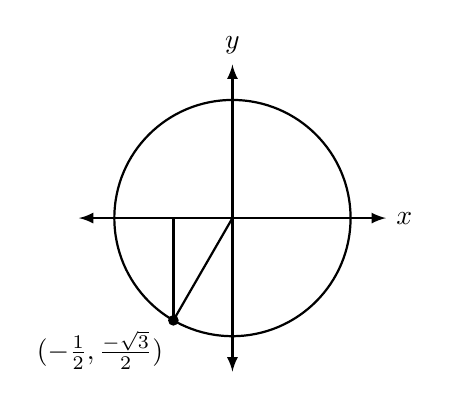
\begin{tikzpicture}[>=latex,scale=1.5,thick]
\draw [<->](-1.3,0)--(1.3,0) node [right] {$x$};
\draw [<->] (0,-1.3) -- (0,1.3) node [above] {$y$};
\draw (0,0) circle (1);
\draw [fill= black] (-.5,-.866) circle (1pt);
\draw (0,0) -- (-.5,-.866) node [below left] {$(-\frac{1}{2}, \frac{-\sqrt{3}}{2})$};
\draw (-.5,-.866) -- (-.5,0);
\end{tikzpicture}

